% Pengaturan ukuran teks dan jenis dokumen
\documentclass[11pt]{article}

% Pengaturan ukuran halaman dan margin
\usepackage[a4paper,top=30mm,left=30mm,right=20mm,bottom=20mm]{geometry}

% Pengaturan ukuran spasi
\usepackage[singlespacing]{setspace}

% Judul dokumen
\title{Proposal Tugas Akhir ITS}
\author{Fadhurrahman, Farhan}

% Pengaturan format bahasa
\usepackage[indonesian]{babel}

% Pengaturan detail pada file PDF
\usepackage[pdfauthor={\@author},bookmarksnumbered,pdfborder={0 0 0}]{hyperref}

% Pengaturan jenis karakter
\usepackage[utf8]{inputenc}

% Pengaturan ukuran indentasi
\setlength{\parindent}{2em}

% Package lainnya
\usepackage{etoolbox} % Mengubah fungsi default
\usepackage{enumitem} % Pembuatan list
\usepackage{lipsum} % Pembuatan template kalimat
\usepackage{graphicx} % Input gambar
\usepackage{longtable} % Pembuatan tabel
\usepackage[table,xcdraw]{xcolor} % Pewarnaan tabel
\usepackage[numbers]{natbib} % Kutipan artikel
\usepackage{changepage} % Pembuatan teks kolom
\usepackage{multicol} % Pembuatan kolom ganda
\usepackage{multirow} % Pembuatan baris ganda

% Pengaturan format judul bab
\usepackage{titlesec}
\renewcommand{\thesection}{\arabic{section}}
\titleformat*{\section}{\normalsize\bfseries}
\titleformat*{\subsection}{\normalsize\bfseries}
\titlespacing{\section}{0ex}{3ex}{1.5ex}
\titlespacing{\subsection}{0ex}{3ex}{1.5ex}

% Isi keseluruhan dokumen
\begin{document}

  % Menonaktifkan penomoran halaman
  \pagenumbering{gobble}

  % Lembar pengesahan
  \begin{flushleft}
  % Ubah kalimat berikut sesuai dengan nama departemen dan fakultas
  \textbf{Departemen Teknik Komputer - FTEIC}\\
  \textbf{Institut Teknologi Sepuluh Nopember}\\
\end{flushleft}

\begin{center}
  % Ubah detail mata kuliah berikut sesuai dengan yang ditentukan oleh departemen
  \underline{\textbf{EC184701  - PRA TUGAS AKHIR - 2 SKS}}
\end{center}

\begin{adjustwidth}{-0.2cm}{}
  \begin{tabular}{lcp{0.7\linewidth}}

    % Ubah kalimat-kalimat berikut sesuai dengan nama dan NRP mahasiswa
    Nama Mahasiswa &:& Farhan Fadhurrahman \\
    NRP &:& 0721 18 4000 0066 \\

    % Ubah kalimat berikut sesuai dengan semester pengajuan proposal
    Semester &:& Ganjil 2021/2022 \\

    % Ubah kalimat-kalimat berikut sesuai dengan nama-nama dosen pembimbing
    Dosen Pembimbing &:& 1.  Dr. Supeno Mardi Susiki Nugroho, S.T., M.T. \\
    & & 2. Reza Fuad Rachmadi, S.T., M.T., Ph.D \\

    % Ubah kalimat berikut sesuai dengan judul tugas akhir
    Judul Tugas Akhir &:& \textbf{Evaluasi Performa Sistem Deteksi Penggunaan Helm pada Pengendara Motor Menggunakan YOLO}\\

    Uraian Tugas Akhir &:& \\
  \end{tabular}
\end{adjustwidth}

% Ubah paragraf berikut sesuai dengan uraian dari tugas akhir
Helm merupakan sebuah alat pelindung yang berfungsi untuk melindungi kepala saat
terjadi benturan. Pada sebuah penelitian didapatkan bahwa menggunakan Helm saat
mengendarai sepeda motor, dapat mengurangi resiko cedera dari kecelakaan lalu lintas
hingga 42\% \citep{helmetUse}. Berdasarkan data dari Badan Pusat Statistik (BPS), jumlah korban
meninggal dalam kasus kecelakaan lalu lintas di Indonesia sebanyak 25.671 jiwa pada
tahun 2019. Pertumbuhan jumlah korban jiwa setiap tahun terus bertambah dengan
persentase hingga 1.41\% \citep{transportasi2019}. Dari latar belakang tersebut, masalah yang dapat diambil
adalah deteksi pengendara Sepeda Motor yang tidak menggunakan helm saat berkendara
yang tidak terdeteksi secara menyeluruh. Oleh sebab itu, diperlukan sebuah sistem untuk
mendeteksi pengendara Sepeda Motor yang tidak menggunakan helm untuk dikembangkan
dalam mendeteksi pelanggar yang tidak menggunakan helm. Dari latar belakang tersebut,
masalah yang dapat diambil adalah deteksi pengendara Sepeda Motor yang tidak
menggunakan helm saat berkendara yang tidak terdeteksi secara menyeluruh. Oleh sebab
itu, diperlukan sebuah sistem untuk mendeteksi pengendara Sepeda Motor yang tidak
menggunakan helm untuk dikembangkan dalam mendeteksi pelanggar yang tidak
menggunakan helm. Tujuan dari penelitian ini adalah mengembangkan dan mengevaluasi performa dari sistem pendeteksi
penggunaan helm pada pengendara Sepeda Motor dengan metode \emph{You Only Look Once} (YOLO).
\vspace{1ex}

\begin{flushright}
  % Ubah kalimat berikut sesuai dengan tempat, bulan, dan tahun penulisan
  Surabaya, Desember 2021
\end{flushright}
\vspace{1ex}

\begin{center}

  \begin{multicols}{2}

    Dosen Pembimbing 1
    \vspace{12ex}

    % Ubah kalimat-kalimat berikut sesuai dengan nama dan NIP dosen pembimbing pertama
    \underline{Dr. Supeno Mardi Susiki Nugroho, S.T., M.T.} \\
    NIP. 197003131995121001

    \columnbreak

    Dosen Pembimbing 2
    \vspace{12ex}

    % Ubah kalimat-kalimat berikut sesuai dengan nama dan NIP dosen pembimbing kedua
    \underline{Reza Fuad Rachmadi, S.T., M.T., Ph.D} \\
    NIP. 198504032012121000

  \end{multicols}
  \vspace{6ex}

  Mengetahui, \\
  % Ubah kalimat berikut sesuai dengan jabatan kepala departemen
  Kepala Departemen Teknik Komputer FTEIC - ITS
  \vspace{12ex}

  % Ubah kalimat-kalimat berikut sesuai dengan nama dan NIP kepala departemen
  \underline{Dr. Supeno Mardi Susiki Nugroho, S.T., M.T. } \\
  NIP. 197003131995121001

\end{center}

  \newpage

  % Konten pendahuluan
  \section{PENDAHULUAN}

\subsection{Latar Belakang}

% Ubah paragraf-paragraf berikut sesuai dengan latar belakang dari tugas akhir
Helm merupakan sebuah alat pelindung yang berfungsi untuk melindungi kepala saat
terjadi benturan. Pada sebuah penelitian didapatkan bahwa menggunakan Helm saat
mengendarai sepeda motor, dapat mengurangi resiko cedera dari kecelakaan lalu lintas
hingga 42\% \citep{helmetUse}. Berdasarkan data dari Badan Pusat Statistik (BPS), jumlah korban
meninggal dalam kasus kecelakaan lalu lintas di Indonesia sebanyak 25.671 jiwa pada
tahun 2019. Pertumbuhan jumlah korban jiwa setiap tahun terus bertambah dengan
persentase hingga 1.41\% \citep{transportasi2019}. Tingginya jumlah korban meninggal dunia pada kecelakaan
lalu lintas diikuti dengan tingginya jenis pelanggaran yang sering dilakukan salah satunya
adalah tidak menggunakan helm oleh pengendara sepeda motor pada saat berkendara \citep{kecelakaan}.

Salah satu penyebab dari tingginya angka kecelakaan pada pengendara sepeda motor adalah keterbatasan
jumlah anggota polisi dalam memantau lalu-lintas sehingga sering terjadi kelalaian pemantauan dan penindakan
pengendara sepeda motor yang tidak menggunakan helm. Oleh karena itu sistem deteksi penggunaan helm pada pengendara
sepeda motor penting, dengan menggunakan teknologi untuk mendapatkan informasi pengendara sepeda motor yang tidak 
menggunakan helm saat berkendara.

Teknologi Visi Komputer adalah sebuah bidang kecerdasan buatan atau Artificial
Intelligence (AI) yang melatih sebuah komputer agar dapat memahami sesuatu dari input
visual. Teknologi Visi Komputer memanfaatkan input dari gambar digital menggunakan
kamera dan jaringan neural atau Neural Network  untuk mengklasifikasikan objek
kemudian dapat mendeteksi sesuatu yang ditangkap oleh komputer. Teknologi Visi
Komputer saat ini sudah banyak diimplementasikan dalam berbagai bidang seperti
administrasi, Kesehatan sampai dengan Transportasi.

\subsection{Rumusan Masalah}

% Ubah paragraf berikut sesuai dengan rumusan masalah dari tugas akhir
Permasalahan yang dapat dirumuskan pada penelitian ini adalah yang pertama deteksi pengendara 
Sepeda Motor yang tidak menggunakan helm saat berkendara tidak terdeteksi secara
menyeluruh. Sehingga diperlukan sebuah sistem dengan performa yang baik untuk mendeteksi pengendara
Sepeda Motor yang tidak menggunakan helm untuk dikembangkan dalam mendeteksi
pelanggar yang tidak menggunakan helm.

\subsection{Penelitian Terkait}

% Ubah paragraf berikut sesuai dengan penelitian lain yang terkait dengan tugas akhir
Hanhe Lin et al dalam artikel penelitiannya yang berjudul \emph{"Helmet Use Detection of Tracked Motorcycles
Using CNN-Based Multi-Task Learning"} pada tahun 2019 mengembangkan sebuah sistem pendeteksi helm
pada pengendara sepeda motor yang berlokasi di beberapa kota negara Myanmar menggunakan metode RetinaNet yang merupakan
sebuah metode \emph{single-stage} untuk mendeteksi sebuah objek. Dalam penilitian ini didapatkan
\emph{mean Average Precision} sebesar 95.3\% \citep{hanhelin}.

Yusuf Umar Hanafi dalam buku tugas akhirnya yang berjudul "Deteksi Penggunaan Helm pada Pengendara Bermotor Berbasis
Deep Learning" pada tahun 2020 membuat sebuah sistem pendeteksi helm menggunakan metode \emph{You Look Only Once} (YOLO). Data input
yang digunakan adalah rekaman video CCTV lalu lintas milik Dinas Perhubungan kota Surabaya. Pengujian dilakukan berdasarkan lokasi,
kondisi, dan objek pelanggar. Pada pengujian ini didapatkan \emph{mean Average Precision} yang cukup baik untuk YOLOv3 \citep{masYusuf}.


\subsection{Tujuan Penelitian}

% Ubah paragraf berikut sesuai dengan tujuan penelitian dari tugas akhir
Tujuan dari penelitian ini adalah:

\begin{enumerate}[nolistsep]

  \item Mengembangkan sistem deteksi penggunaan helm pada pengendara motor menggunakan metode YOLO.
  \item Mengevaluasi performa dari metode YOLO dalam mendeteksi penggunaan helm pada pengendara sepeda motor.

\end{enumerate}


  % Konten tinjauan pustaka
  \section{TINJAUAN PUSTAKA}

% Ubah konten-konten berikut sesuai dengan isi dari tinjauan pustaka

\subsection{Hukum Newton}

% Contoh penggunaan referensi dari pustaka
Newton pernah merumuskan \citep{Newton1687} bahwa \lipsum[8]
% Contoh penggunaan referensi dari persamaan
Kemudian menjadi persamaan seperti pada persamaan \ref{eq:FirstLaw}.

% Contoh pembuatan persamaan
\begin{equation}
  % Label referensi dari persamaan yang dibuat
  \label{eq:FirstLaw}
  % Baris kode persamaan yang dibuat
  \sum \mathbf{F} = 0\; \Leftrightarrow\; \frac{\mathrm{d} \mathbf{v} }{\mathrm{d}t} = 0.
\end{equation}

\lipsum[9]

\subsection{Anti Gravitasi}

\lipsum[10]


  % Konten metodologi
  \section{METODOLOGI}

% Ubah konten-konten berikut sesuai dengan isi dari metodologi

\subsection{Dataset yang Digunakan}

Data yang digunakan adalah video yang direkam pada beberapa jalan di kota Surabaya lalu
diekstrak menjadi gambar yang akan dianotasikan sesuai dengan format \emph{bounding box}
YOLO.

% Contoh input gambar dengan format *.jpg
\begin{figure} [ht] \centering
  % Nama dari file gambar yang diinputkan
  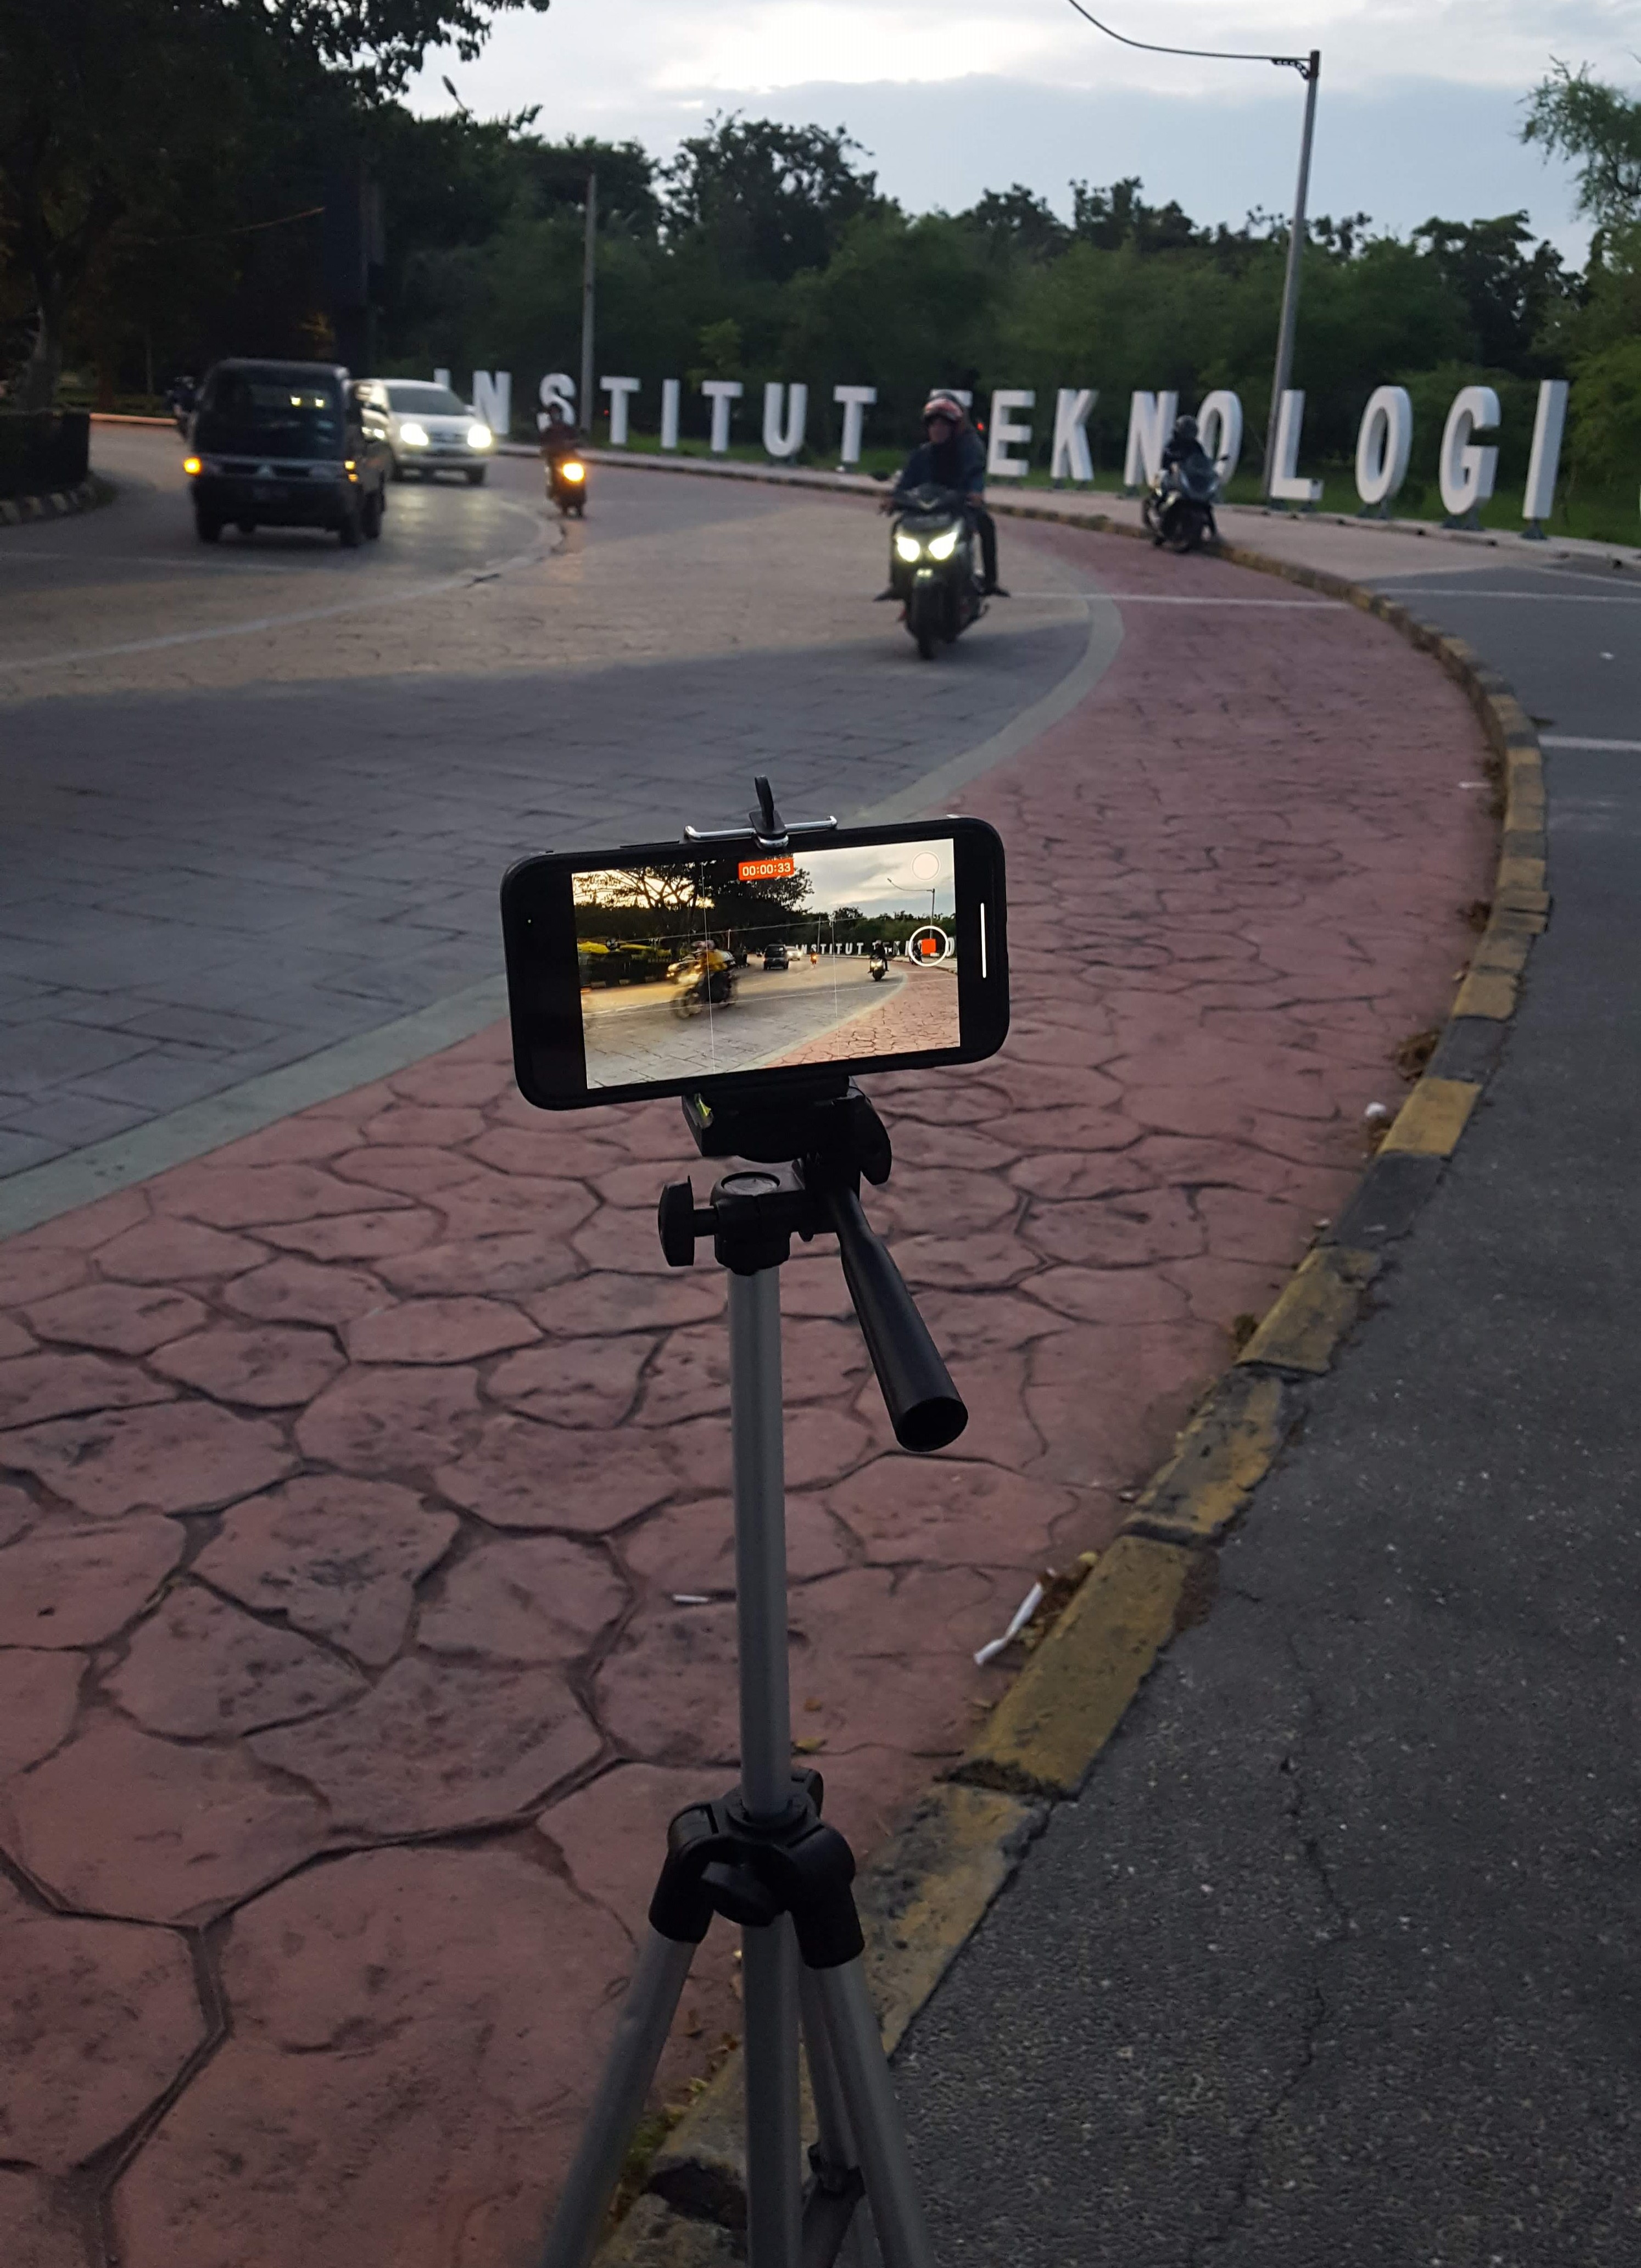
\includegraphics[scale=0.05]{gambar/pengambilan-vide.jpg}
  % Keterangan gambar yang diinputkan
  \caption{Posisi kamera dalam mengambil data video}
  % Label referensi dari gambar yang diinputkan
  \label{fig:pengambilan-video}
\end{figure}

% Contoh penggunaan referensi dari gambar yang diinputkan
Pada tahap pengambilan data video, data video diambil menggunakan kamera pada \emph{smartphone} Apple Iphone XS yang diletakkan pada tepi beberapa jalan raya di kota Surabaya. Kamera \emph{smartphone}
diletakkan pada \emph{tripod} yang memiliki tinggi 1,5 meter. Posisi peletakan kamera pada tripod bisa dilihat pada Gambar \ref{fig:pengambilan-video}.
Setiap video yang diambil menggunakan resolusi 1920 x 1080 \emph{pixels} 30 \emph{frame per second} dengan durasi setiap video 20 menit.


\subsection{Metodologi Penelitian}

Penelitian ini dilaksanakan sesuai sistem berikut dengan implementasinya. Desain
sistem merupakan konsep dari pembuatan dan perancangan infrastuktur yang kemudian diwujudkan
dalam bentuk blok diagram alur yang harus dikerjakan. Pada bagian implementasi merupakan
pelaksanaan teknis untuk setiap blok pada desain sistem. Pada Gambar \ref{fig:diagram-alur} menunjukan bagan umum metodologi
sistem.

\begin{figure} [ht] \centering
  % Nama dari file gambar yang diinputkan
  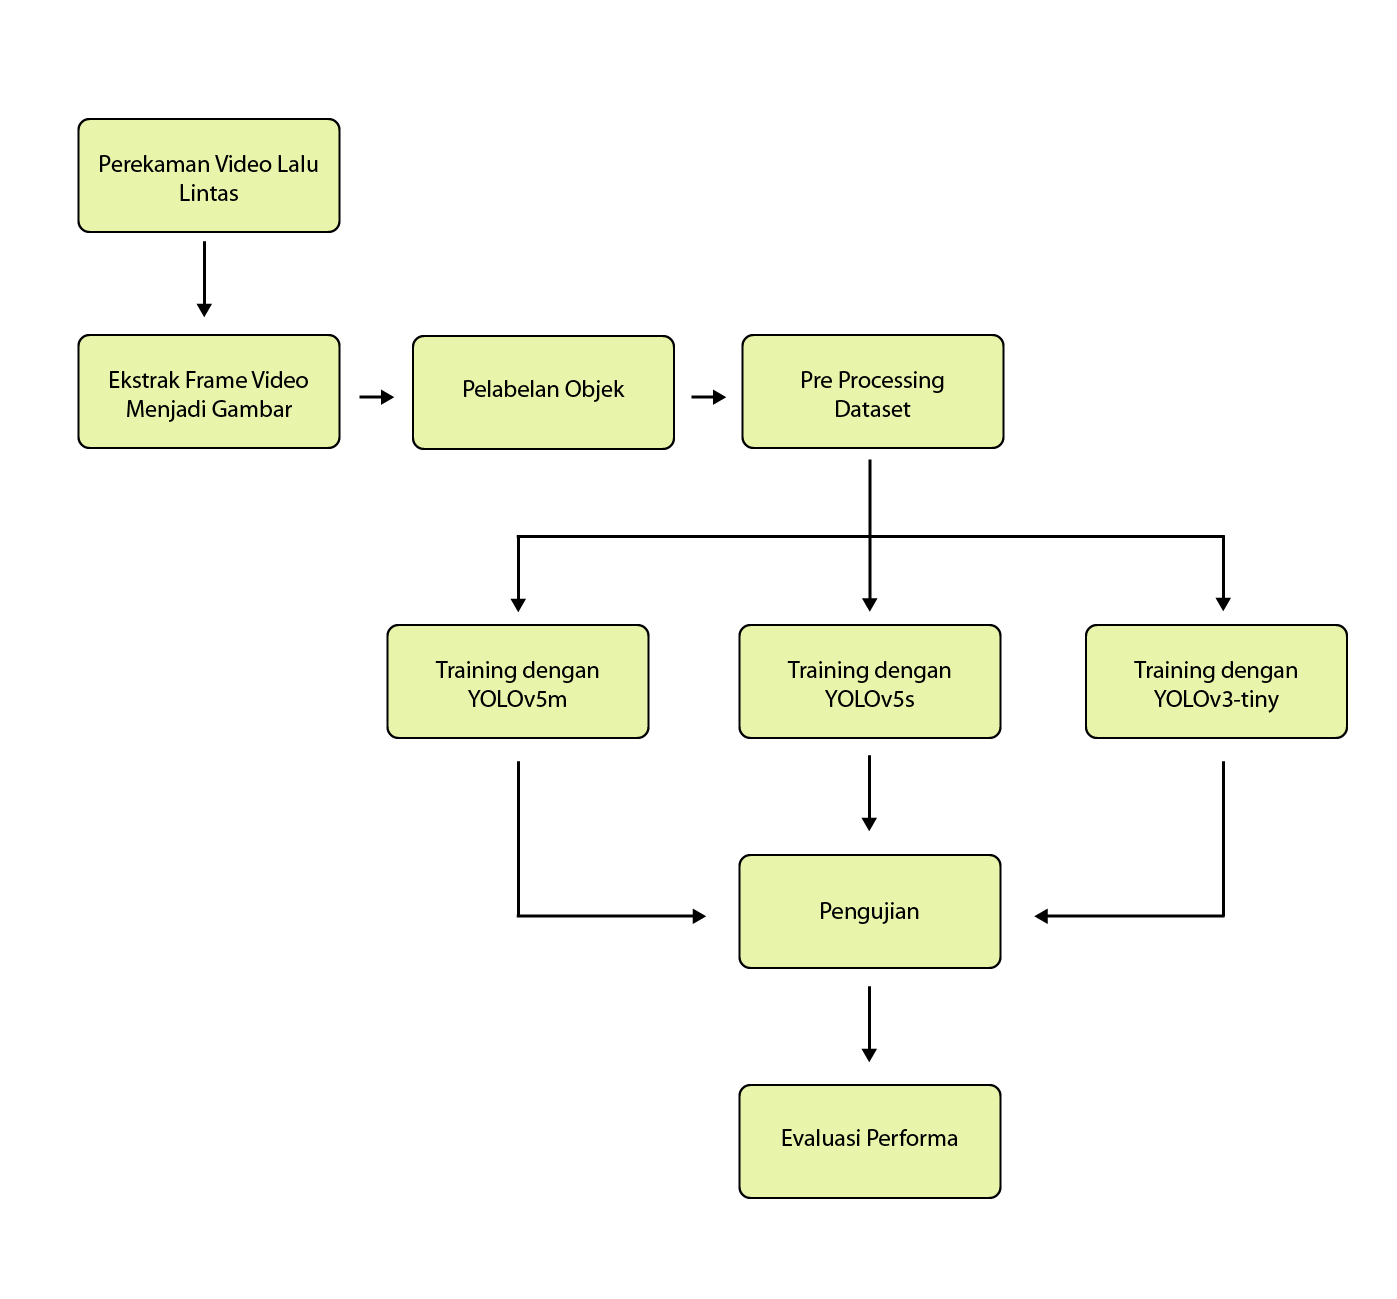
\includegraphics[scale=0.25]{gambar/diagram-pengerjaan-2-100.jpg}
  % Keterangan gambar yang diinputkan
  \caption{Diagram Alur Pengerjaan}
  % Label referensi dari gambar yang diinputkan
  \label{fig:diagram-alur}
\end{figure}

Berdasarkan pada bagan alur metodologi yang dapat dilihat pada Gambar \ref{fig:diagram-alur}, Tahapan pertama yang dilakukan adalah
perekaman video kondisi lalu lintas kota Surabaya. Perekaman video tersebut dilakukan menggunakan perangkat \emph{smartphone} Apple Iphone XS.
Tujuan dari perekaman video tersebut adalah untuk mengumpulkan data yang dibutuhkan untuk proses \emph{training} dan pengujian sistem dari metode yang digunakan.
Dalam sistem ini terdapat tiga objek yang akan dideteksi yaitu adalah pengendara sepeda motor, kepala pengendara sepeda motor menggunakan helm dan kepala pengendara 
sepeda motor tanpa menggunakan helm. Lalu objek tersebut diberikan label atau anotasi yang sesuai kelas yang ditambahkan. Pelabelan data tersebut berupa
\emph{bounding box} yang menunjukkan posisi kelas objek tersebut berdasarkan koordinat resolusinya. Setelah didapatkan data yang lengkap dengan labelnya, lalu data tersebut dapat digunakan
pada proses \emph{training} menggunakan metode deteksi objek berbasis CNN yaitu YOLOv5 dan YOLOv3. \emph{Weight} yang digunakan pada YOLOv5 adalah YOLOv5m dan YOLOv5s, sedangkan
untuk YOLOv3 menggunakan YOLOv3-tiny.


  % Konten lainnya
  \section{HASIL YANG DIHARAPKAN}

\subsection{Hasil yang Diharapkan dari Penelitian}

Dari penelitian yang akan dilakukan, diharapkan \lipsum[15]

\subsection{Hasil Pendahuluan}

Sampai saat ini, kami telah \lipsum[16]

\section{RENCANA KERJA}

% Ubah tabel berikut sesuai dengan isi dari rencana kerja
\newcommand{\w}{}
\newcommand{\G}{\cellcolor{gray}}
\begin{table}[h!]
  \begin{tabular}{|p{3.5cm}|c|c|c|c|c|c|c|c|c|c|c|c|c|c|c|c|}

    \hline
    \multirow{2}{*}{Kegiatan} & \multicolumn{16}{|c|}{Minggu} \\
    \cline{2-17} &
    1 & 2 & 3 & 4 & 5 & 6 & 7 & 8 & 9 & 10 & 11 & 12 & 13 & 14 & 15 & 16 \\
    \hline

    % Gunakan \G untuk mengisi sel dan \w untuk mengosongkan sel
    Pengambilan data &
    \G & \G & \G & \G & \w & \w & \w & \w & \w & \w & \w & \w & \w & \w & \w & \w \\
    \hline

    Pengolahan data &
    \w & \w & \w & \w & \G & \G & \G & \G & \w & \w & \w & \w & \w & \w & \w & \w \\
    \hline

    Analisa data &
    \w & \w & \w & \w & \w & \w & \w & \w & \G & \G & \G & \G & \w & \w & \w & \w \\
    \hline

    Evaluasi penelitian &
    \w & \w & \w & \w & \w & \w & \w & \w & \w & \w & \w & \w & \G & \G & \G & \G \\
    \hline

  \end{tabular}
\end{table}


  % Daftar pustaka
  \section{DAFTAR PUSTAKA}
  \renewcommand\refname{}
  \vspace{-2ex}
  \bibliographystyle{unsrtnat}
  \bibliography{pustaka/pustaka.bib}

\end{document}
